\documentclass[12pt]{article}
\usepackage[landscape]{geometry}
\usepackage{graphicx,color} 
\include{def.tex}


\begin{document}
\pagestyle{empty}

\noindent A parallel plate capacitor has two plates has a separation $d$ and capacitance, $C$.  If I charge it with a $+Q$ and a $-Q$ on the two plates, respectively, what is the electrostatic energy? What is it if I move the two plate closer together to $d/2$?  How would the answer differ if I maintain a constant potential difference, $\Delta V$ between the two?

\newpage

\noindent Consider the following parallel plate capacitor that is half-filled with two different dielectrics.  The seperation between the two capacitors is $d$.  What is the equivalent capacitance if material $k_1$ fills 1/3 the space of $k_2$?

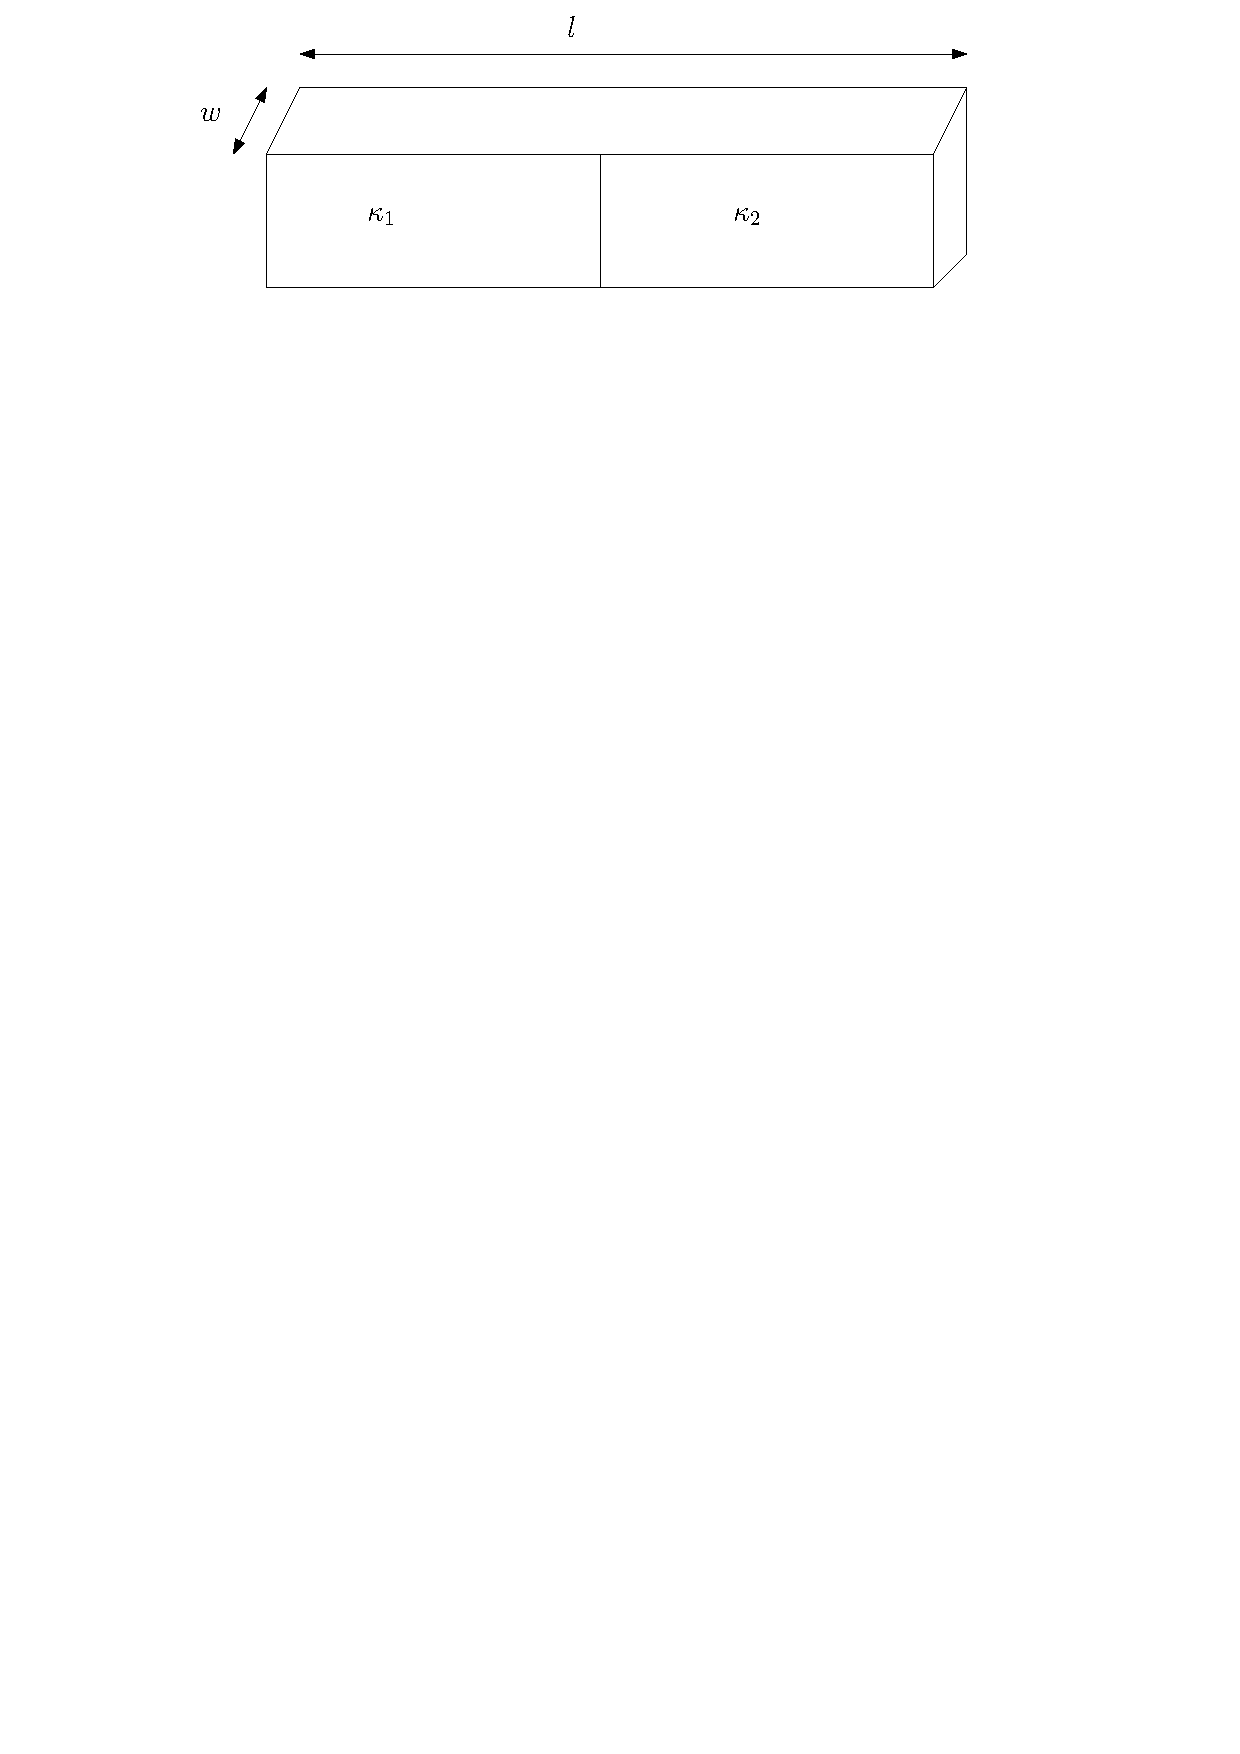
\includegraphics[width=0.4\textwidth]{two-dielectric.pdf}

\newpage 


\noindent Suppose a spherical capacitor that consists of two conducting shells of with radii $a$ and $b$ and $a > b$. If a charge $+Q$ is placed on the outer shell and $-Q$ on the inner shell, what is the electrostatic energy between the two shells.  

\newpage 

\noindent Consider the following arrangements of identical capacitors, with capacitance $C_0$.  What is is the equivalent capacitance between a and b?

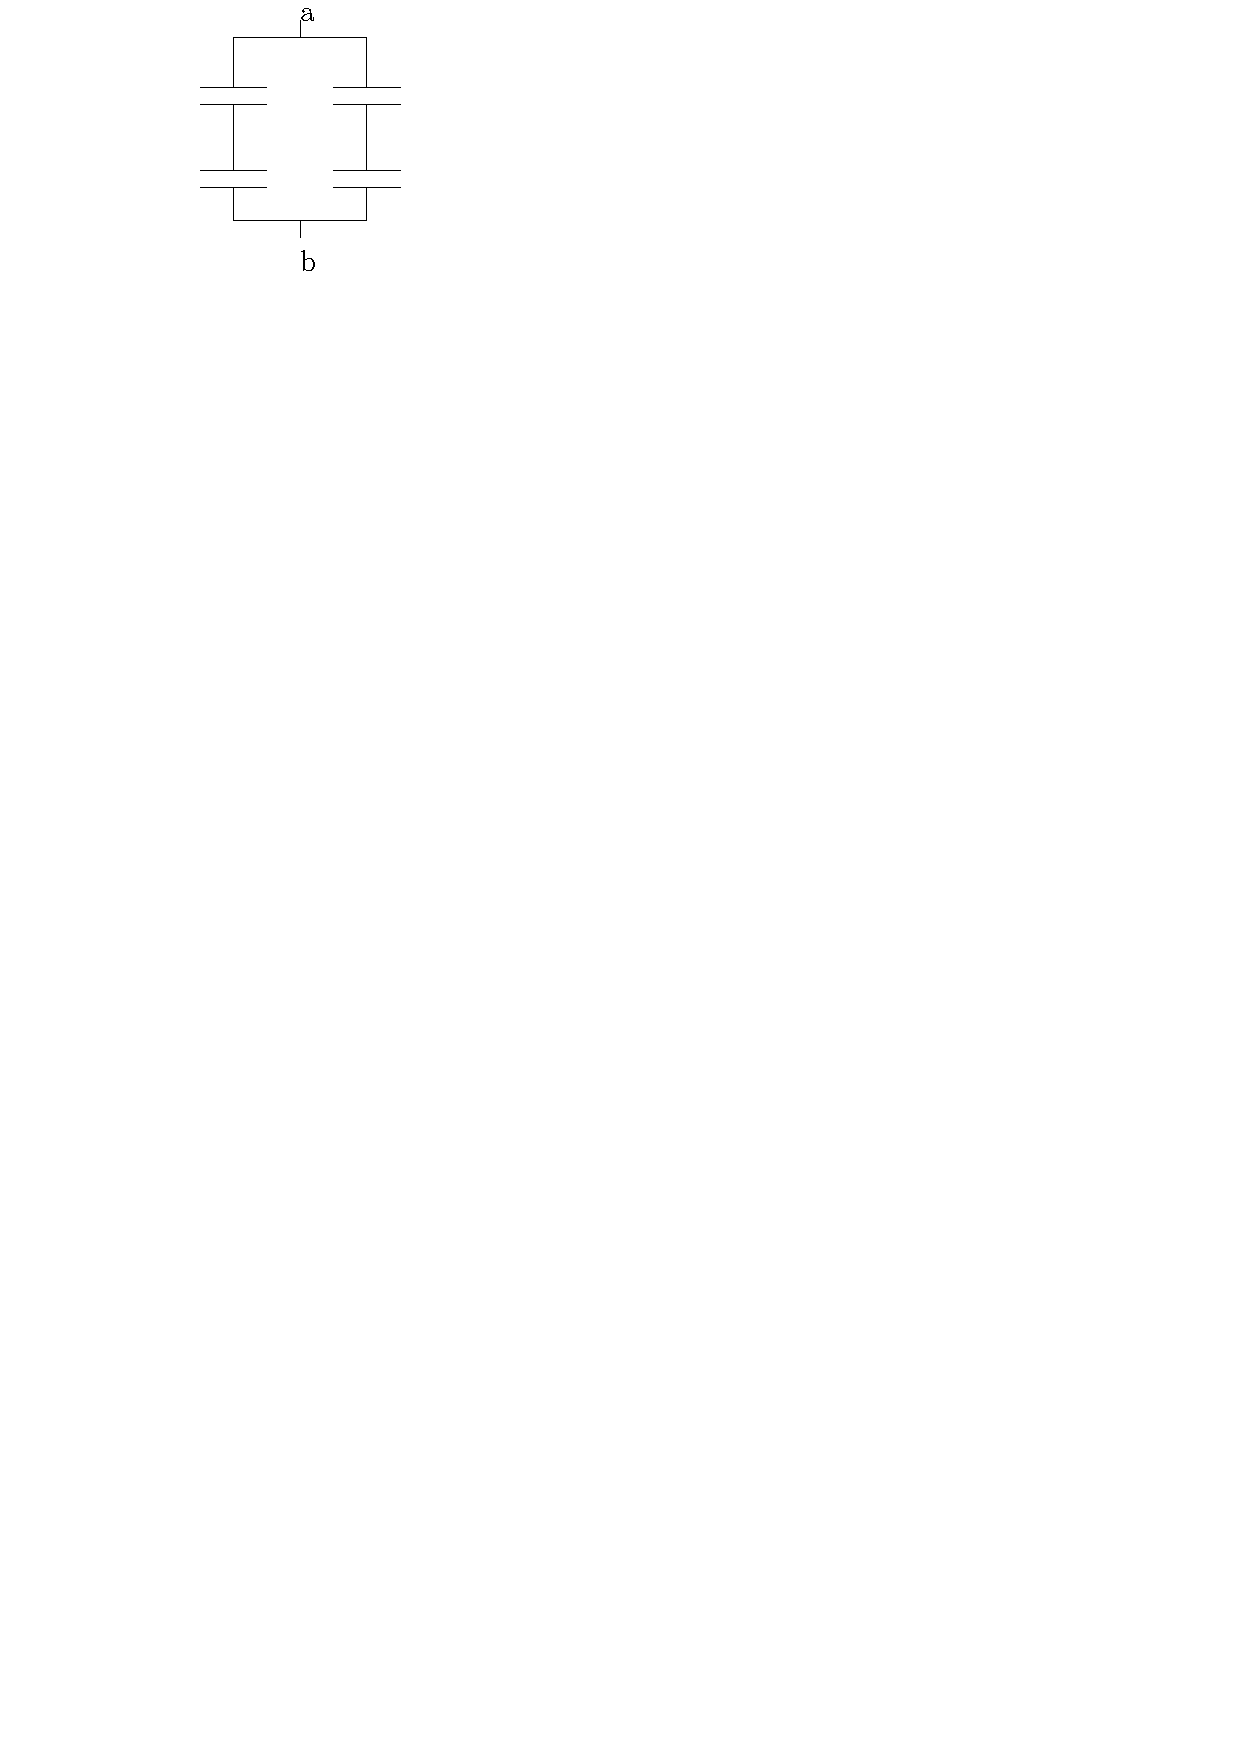
\includegraphics[width=0.25\textwidth]{capacitor-circuit.pdf}

\end{document}
